\documentclass{article}
\usepackage[utf8]{inputenc}
\usepackage{graphicx}
\usepackage{epstopdf}
\graphicspath{{./images/}}
\usepackage{caption}
\usepackage[english]{babel}
\usepackage{amsmath,amssymb,amsthm}
\usepackage{a4wide}
\usepackage{tikz}
\usetikzlibrary{calc}
\title{Description Capita Selecta}
\author{Omar Richardson}
\let\oldhat\hat
\let\oldtil\tilde
\DeclareMathOperator{\diag}{diag}
\DeclareMathOperator{\D}{D}
\renewcommand{\vec}[1]{\mathbf{#1}}
\newcommand{\gvec}[1]{\boldsymbol#1}
\renewcommand{\tilde}[1]{\oldtil{\mathbf{#1}}}
\newcommand{\eps}{\varepsilon}
\newcommand{\bigo}[1]{\mathcal{O}\left(#1\right)}
\newtheorem{newdef}{Definition}
\newtheorem{newthm}{Theorem}
\begin{document}

\maketitle

\section{Abstract}
Crowd dynamics is an emerging field of research. With more computational power and algorithms available, realistic crowd simulations become better and better. When desiring to model a crowd, several dependable modelling options are available. Some models employ stochastic differential equations to model the movements of agents as Brownian motions. Other models represent the agents as occupied cells on a grid.
\ \\
These ways of modelling has proven to work well for small crowds. When crowds become dense, other options become available as well. One of these options is to combine both a global as a local approach in the model, where the global approach models the crowd as a fluid, and the local approach models agents as individual agents. Using the right simulation architecture, this way of modelling is able to handle crowds with a large number of agents at a relatively low computational cost.

\ \\
The goal of this capita selecta is to implement this method and check its performance in the case of a large crowd in need of evacuation. 

\newpage
\section{Implementation overview}
This model is composed of several modules. These modules will be implemented disjointly. This will enable us to swap or upgrade modules without having to adapt the rest, and keep the implementation improvable and maintainable.
\begin{enumerate}
	\item \textbf{Geometry}\\
	This part models the scenario in which the agents are placed, the obstacles they have to avoid, and the goal they are headed to.
	\item \textbf{Global planner}\\
	This module determines the paths of the agents that brings them to their goal. From these destinations and the geometry, it determines the desired speed and direction of every agent.
	\item \textbf{Continuum aspects}\\
	This module converts the agents mass and velocity to a global density and velocity field, which will be used to influence the agents individual velocity. 
	This module also applies a incompressibility constraint to the global representation to ensure local densities do not exceed a maximum.
\end{enumerate}
The model will be implemented in Python. Motivation behind this language is that it has dependable scientific computing libraries available, like \texttt{numpy} and \texttt{scipy}. It also has the advantage of an object oriented structure, which will make working with agents on a local level more manageable.
\newpage
\section{Geometry}
This section will elaborate on the implementation of the geometry.
\subsection{Summary}
The geometry consists of a scene filled with multiple obstacles. The scene is the domain of calculation. It is modelled as a rectangle, surrounded with walls and exits. Within this domain, agents are spawned, trying to make their way to the exit while dodging the obstacles (and each other). an agent will be eliminated once he has made his way to the exit.

\subsection{Structure}
The geometry is divided into a computational component and a visual component. The computational component handles the computations of the next time step of the scene. The visual component acts separately and displays the geometry (and the agents) at every time step. This part can be suppressed to increase simulation capacity.

\subsection{Obstacles}
The scene can be filled with an arbitrary number of objects, provided that all agents spawned are able to reach the exit given their initial location. The objects all have a rectangular shape. This choice is motivated by their relative ease in modelling and calculating. In addition, rectangular objects can easily be aggregated to more general shapes.
\ \\
A scene contains both an entrance and an exit. The entrance is modelled as an obstacle with a certain \underline{inflow} of agents (this allows us to imitate a PDE-like boundary condition) and the exit is modelled as a penetrable obstacle. By default, a scene is surrounded by walls. Whenever an exit or entrance is defined, it replaces the walls.
\subsection{Agents}
The agents are modelled as particles with a position and a velocity. The agents are able to assume any position in the scene where no obstacles are present. Agents can only leave the scene through an exit.
The agents have a maximum speed, randomly drawn from a specified interval.

\ \\
The agents are displayed in the geometry by colored circles. Optionally, it is possible to display the agents as directed triangles, to indicate their movement direction.
\newpage
\section{Global planner}
\subsection{Summary}
This section describes the global planner module. The planner has the objective of planning a path for every agent to follow that will lead him to his goal. This path has to avoid the obstacles in the scene but ignores the position of other agents. Collisions with other agents will be avoided by the continuum solver. We elaborate on this module in Section \ref{sec:continuum}.

\ \\
In this implementation, we combine line segments to form piecewise linear paths. The path taken is the shortest path to the exit avoiding the obstacles. An example of a planned agent path is provided in Figure \ref{fig:example_path}. We compute a path by representing the scene as a weighted graph and determining the shortest path from the agents position to the exit.
\begin{figure}[h]
	\centering
	\includegraphics{images/example_graph.png}
	\caption{An example of a scene geometry and the corresponding path planned out for the agent.}
	\label{fig:example_path}
\end{figure}
\subsection{Graph representation}
We will explain the algorithm by example. We model our scene as a two-dimensional set $\Omega \subset \mathbb{R}^2$. In this set, we have obstacles $M_i \subset \Omega$ and location of agents $a_j$ as points $(x_{a_j},y_{a_j}) \in \Omega$. 
\begin{newdef}
	Let $M \subset \Omega$ be a rectangular obstacle with lower left corner $\vec{s}=(s_x,s_y)$ and upper right corner $\vec{t}=(t_x,t_y)$. The shape of this obstacle is denoted as $[\vec{s},\vec{t}]$. The four corner points (lower-left, lower-right, upper-left and upper-right) are denoted respectivily as $\vec{m}^{00},\vec{m}^{10},\vec{m}^{01},\vec{m}^{11}$ and have values
	\begin{align}
		\vec{m}^{00}&=(s_x,s_y)\\
		\vec{m}^{10}&=(t_x,s_y)\\
		\vec{m}^{01}&=(s_x,t_y)\\
		\vec{m}^{11}&=(t_x,t_y)
		\label{eq:corner_points}
	\end{align}
\end{newdef}
In Figure \ref{fig:example_path} we see an illustration of a scene $\Omega$ of size $R_x\times R_y$ containing $N_o = 2$ obstacles $M_1$ and $M_2$ with shapes $[\vec{s}_{M_1},\vec{t}_{M_1}]$ and $[\vec{s}_{M_2},\vec{t}_{M_2}]$. We seek a path for agent $a$ at location $\vec{x}_a$ to the exit $E$.

\ \\
Let $G = (V,A)$ be a weighted, undirected graph. 
Our vertex set $V$ is constructed by joining the set of all corner points with the pedestrian location and the exit.
\begin{equation}
	V = \left\{\left.\vec{m}^{ij}_k \right| i,j \in \{0,1\}, k = 1,\dots,N_o \right\} \cup \{E,a\}
	\label{eq:vertex_set_construction}
\end{equation}

\ \\
For each two nodes $v_i,v_j\in V$ we add edge $(v_i,v_j)$ to edge set $A$ if and only if the line segment between these points is contained in $\Omega$ and unhindered by other obstacles. The algorithm used to deduce whether a path is free of obstacles is described in Section \ref{sec:crosses_obstacle}. We choose the weight of the edge equal to the distance between the nodes. The result is a graph as depicted in Figure \ref{fig:example_graph}.

\ \\
We chose to model the exit obstacle as a single node. This is motivated by wanting the pedestrians to find the fastest way to leave the scene, and we do not want to restrict their paths to the corners of the exit. The distance between an obstacle corner point and the exit is computed as the distance between a point and a set.
\begin{figure}[h]
	\centering
	\includegraphics[width=0.7\textwidth]{images/obstacle_graph.pdf}
	\caption{Example of the weighted graph corresponding to the scene in Figure \ref{fig:example_path}. The unmarked nodes correspond to the corners of the obstacles.}
	\label{fig:example_graph}
\end{figure}\\
In Figure \ref{fig:example_graph} we see the complete graph representation of the scene. Now, any path from node $\vec{x}_a$ to exit $E$ is a feasible path free of obstacles, since the edges are not hindered by obstacles.

\ \\
After obtaining this graph, we apply the $A^*$-algorithm to the graph to find the shortest path from $\vec{x}_a$ to $E$ and store it.
\newpage
\subsection{Determining hindering obstacles}
\label{sec:crosses_obstacle}
To find whether a line segment is free of obstacles, we use some basic linear algebra. Specifically, we use hyperplanes and \emph{bounding rectangles}. 
\ \\
First, some definitions:
\begin{newdef}
	Let $\Omega \in \mathbb{R}^2$ be a scene.
	Let $l\subset \Omega$ be a line segment from $\vec{p}$ to $\vec{q}$ with $\vec{p},\vec{q} \in \mathbb{R}^2$. Then the corresponding hyperplane $L$ (i.e., the hyperplane that covers the line segment) is defined as the set of all $\vec{x}\in\mathbb{R}^2$ satisfying
	\begin{equation}
		(\vec{a},\vec{x})=b
	\end{equation}
	where $\vec{a}$ and $b$ equal 
	\begin{align}
		\vec{a} &= \left( -(p_y-q_y),(p_x-q_x)\right)\\
		b   &=  p_y(p_x - q_x) - p_x(p_y - q_y)
	\end{align}
\end{newdef}
\noindent
A hyperplane separates the set $\Omega$ into two sets $\Omega_{L^+}$ and $\Omega_{L^-}$ such that
\begin{align}
\Omega = \Omega_{L^+} \cup \Omega_{L^-} \cup L\\
\Omega_{L^+}\cap\Omega_{L^+}=\emptyset.
	\label{def:hyp}
\end{align}
It is a simple task to determine whether a point $\vec{x}$ belongs to either one of the subsets (or the hyperplane itself) by computing the inner product with $\vec{a}$.
\begin{newdef}
	Let $\vec{x}$ be a point in $\mathbb{R}^2$. Let $L$ be a hyperplane separating $\Omega$ into subsets $\Omega_{L^+}$ and $\Omega_{L^-}$. These sets are defined in the following way:
	\begin{equation}
		\begin{cases}
			\vec{x} \in L&\mbox{ if }(a,x) = b\\
			\vec{x}  \in \Omega_{L^-} &\mbox{ if }(a,x) < b\\
			\vec{x}  \in \Omega_{L^+} &\mbox{ if }(a,x) > b\\
		\end{cases}
		\label{eq:separation}
	\end{equation}
\end{newdef}
\begin{newdef}
	Let $l$ be a line segment from $\vec{p}$ to $\vec{q}$. The bounding rectangle $P_l$ is defined as the smallest rectangle containing $l$:
	\begin{equation}
		P_l = \left\{ w\in\mathbb{R}^2| \min\{p_x,q_x\} \leq w_x \leq \max\{p_x,q_x\}, \min\{p_y,q_y\} \leq w_y \leq \max\{p_y,q_y\}  \right\}
		\label{eq:bounding_rect}
	\end{equation}
\end{newdef}
\noindent
An example of a bounding rectangle is illustrated in Figure \ref{fig:bounding_rect_ex}.
\begin{figure}
	\centering
	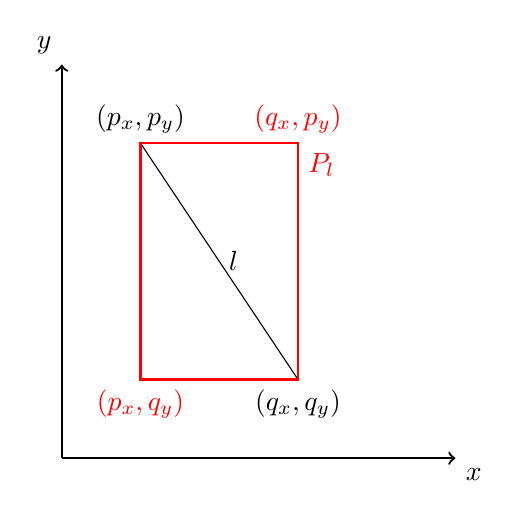
\begin{tikzpicture}
		\draw[step=2cm,black,thin] (1,4) node[anchor=south] {$(p_x,p_y)$} -- node[anchor=west]{$l$} (3,1) node[anchor=north] {$(q_x,q_y)$};
		\draw[thick,red] (1,1) rectangle (3,4) node[anchor=north west]{$P_l$};
		\draw[step=2cm,black,thin] (1,1) node[anchor=north,red] {$(p_x,q_y)$};
		\draw[step=2cm,black,thin] (3,4) node[anchor=south,red] {$(q_x,p_y)$};
		\draw[thick,->] (0,0) -- (5,0) node[anchor=north west] {$x$};
		\draw[thick,->] (0,0) -- (0,5) node[anchor=south east] {$y$};
	\end{tikzpicture}
	\captionof{figure}[Caption]{Line segment $l$ and the corresponding bounding rectangle $P_l$ with shape $[(p_x,q_y),(q_x,p_y)]$}
	\label{fig:bounding_rect_ex}
\end{figure}

\begin{newthm}
	Let $A$ and $B$ be two rectangles with shapes $[\vec{s}_A,\vec{t}_A]$ and $[\vec{s}_B,\vec{t}_B]$. Then the intersection $A\cap B$ is non-empty if and only if
	\begin{equation}
		\vec{t}_{Ai} < \vec{s}_{Bi} \mbox{ or }	\vec{t}_{Bi} < \vec{s}_{Ai}\, \forall i \in \{1,2\}
		\label{eq:intersection}
	\end{equation}
	
\end{newthm}
\begin{newthm}
	Let $l\subset \Omega$ be a line segment and $M \subset \Omega$ be an obstacle. Then the following statements are equivalent:
		\begin{enumerate}
			\item $l \cap M = \emptyset$
			\item $P_l \cap M = \emptyset \mbox{ or } M \subset \Omega_{L^+} \mbox{ or } M \subset \Omega_{L^-}$
		\end{enumerate}
	\label{thm:sep}
\end{newthm}
\begin{proof}
	(2) $\implies$ (1):\\
	Assume $P_l \cap M = \emptyset$. We know $l \subset P_l$ and therefore $l \cap M = \emptyset$.\\
	Otherwise, without loss of generality, assume $M \subset \Omega_{L^+}$. We know $\Omega_{L^+} \cap l = \emptyset$ so $M \cap l = \emptyset$.

	\ \\
	$\neg (2) \implies \neg (1)$:\\
	Assume $P_l \cap M \neq \emptyset,\, M \not\subset \Omega_{L^+} \mbox{ and } M \not\subset \Omega_{L^-}$.\\
	Let $C := P_l \cap M$. $C$ is the intersection of two rectangular sets and therefore rectangular itself.\\
	Let $C^+:=P_l \cap M \cap \Omega^{L^+}$ and $C^-:= P_l \cap M \cap \Omega^{L^-}$. By construction (\emph{needs more argument}), we know $C^+$ and $C^-$ are non-empty sets.
	
	\ \\
	We can pick $\vec{c}^+ \in C^+$ and $\vec{c}^- \in C^-$ and construct line segment $c$ from $\vec{c}^+$ to $\vec{c}^-$. Since $C^+,C^- \subset C$ and $C$ is a convex set, we know $c \subset C$. But since $\vec{c}^+ \in \Omega_{L^+}$ and $\vec{c}^- \in \Omega_{L^-}$ we know $c$ intersects $l$, so $l \cap M \neq \emptyset$.
\end{proof}
\newpage
\noindent
Using these theorems, we have an computationally efficient way to determine the obstacles crossing a line segment.
In Figure \ref{fig:crosses_obstacle} we see an example of an obstacle and a line segment which do not intersect.
Since a rectangle is a convex set, checking $M \subset A$ reduces to checking $\vec{m}^{ij} \in A$ for $i,j \in \{0,1\}$.
\emph{Maybe say something about the efficiency of the calculation}
\\ \
\begin{figure}[ht]
	\centering
	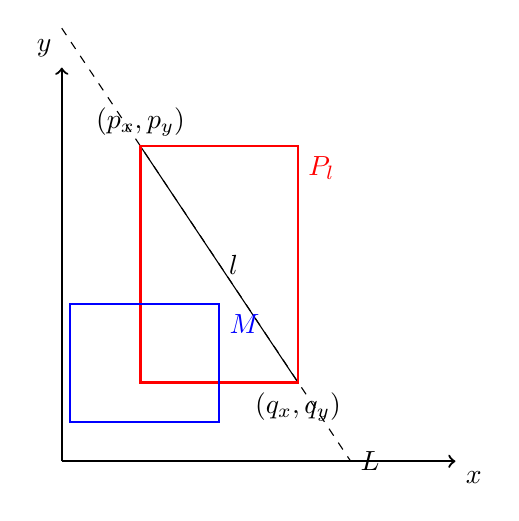
\begin{tikzpicture}
		\draw[step=2cm,black,thin] (1,4) node[anchor=south] {$(p_x,p_y)$} -- node[anchor=west]{$l$} (3,1) node[anchor=north] {$(q_x,q_y)$};
		\draw[step=2cm,black,thin,dashed] (0,5.5) -- (3.67,0) node[anchor=west]{$L$};
		\draw[thick,red] (1,1) rectangle (3,4) node[anchor=north west]{$P_l$};
		\draw[thick,blue] (0.1,0.5) rectangle (2,2) node[anchor=north west]{$M$};
		\draw[thick,->] (0,0) -- (5,0) node[anchor=north west] {$x$};
		\draw[thick,->] (0,0) -- (0,5) node[anchor=south east] {$y$};
	\end{tikzpicture}
	\captionof{figure}[Caption]{Line segment $l$ and obstacle $M$. There is a non-empty intersection between $P_l$ and $M$, but no intersection between $l$ and $M$ because all of $M$ lies on the same side of the hyperplane $L$.}
	\label{fig:crosses_obstacle}
\end{figure}\\
\newpage
\section{Continuum aspects}
\label{sec:continuum}
This section will elaborate on the continuum part of the implementation; converting the agents to a continuum and computing its properties.
\subsection{Overview}
The \underline{continuum solver} uses the following partial differential equation, based on the continuity equation for mass but adapted with a pressure term.
\begin{equation}\label{eq:pde}
\frac{\partial \rho}{\partial t} =-\nabla \cdot(\rho{v}) + \nabla \cdot (\rho\nabla p)
\end{equation}
with scalar density field $\rho(x,y,t)$, vector velocity field $v(x,y,t) = \begin{pmatrix}v_x\\v_y\end{pmatrix}$ and scalar pressure field $p(x,y,t)$.

\ \\
To utilise our fluid flow solver, we need a global representation of the agents. The agents' individual mass and velocity has to be converted to a global density, velocity and pressure. In this implementation, we choose to define a grid of cells over the scene. In each cell, we compute a numerical estimate for each field. Both the density and the velocity of a given cell are interpolated from the agents nearby the cell. Then, using these two fields, we numerically compute the next time step of the pressure and the velocity in \eqref{eq:pde}. Finally, we use these two fields to restrict the motion of the agents.

\ \\
Our fluid solver influences the agents in two ways: 
\begin{itemize}
\item Swarm behaviour
\item Incompressibility
\end{itemize}
\subsubsection{Incompressibility Constraint}
Our incompressibility imposes some restrictions on the density and the velocity. We assume a maximum density $\rho_{\max}$. Wherever our density $\rho(x)$ reaches $\rho_{\max}$, the scene is locally saturated, and the agents have to divert from their path. 

\ \\
\underline{Using variational calculus} we obtain that the optimal $v$ respecting $v_{\max}$ equals $$v = v_{\max}\frac{v-\nabla p}{||v-\nabla p||}.$$
under the constraints that 
\begin{align}
\label{eq:comp}
p>0 \texttt{ OR } \rho=\rho_{\max}\\
p>0 \implies \nabla\cdot v=0
\end{align}
Note that \eqref{eq:comp} implies that $\rho$ and $p$ are complementary variables, i.e. that $\rho(x)p(x)=0$ for all $x$.
\subsubsection{Swarm behaviour}
The solver computes the velocity field of the crowd on a grid. This field influences the individual speed of the agents. When the density in an agents neighbourhood becomes higher, his velocity will converge to the velocity of the crowd. The actual velocity $v_{a_i}$ of agent $a_i$ (located at $(x_{a_i},y_{a_i})$) becomes the average of his desired velocity $\bar{v}_{a_i}$ and the crowds velocity $v(x_{a_i},y_{a_i},\cdot)$, weighted to the local density:
\begin{equation}
	v_{a_i} = \left(1-\frac{\rho(x_{a_i},y_{a_i},\cdot)}{\rho_{\max}}\right)\bar{v}_{a_i}+\frac{\rho(x_{a_i},y_{a_i},\cdot)}{\rho_{\max}}v(x_{a_i},y_{a_i},\cdot)
	\label{eq:dens_velo}
\end{equation}


\subsection{Discretization}
We desire a numerical approximation of $\rho$, $p$ and $v$. To obtain this, we first discretize our domain and our equation. We define a grid of $(N_x,N_y)$ cells, where every cell has a size of $h_x\times h_y$. Our complete scene has dimensions $N_xh_x\times N_yh_y$. 
\ \\
We discretize our scalar and vector fields corresponding to the grid. We index the cells (and the fields) from the bottom left, corresponding with the Carthesian coordinate system in the scene. This is illustrated in Figure \ref{fig:indexing}.
\begin{figure}
	\centering
	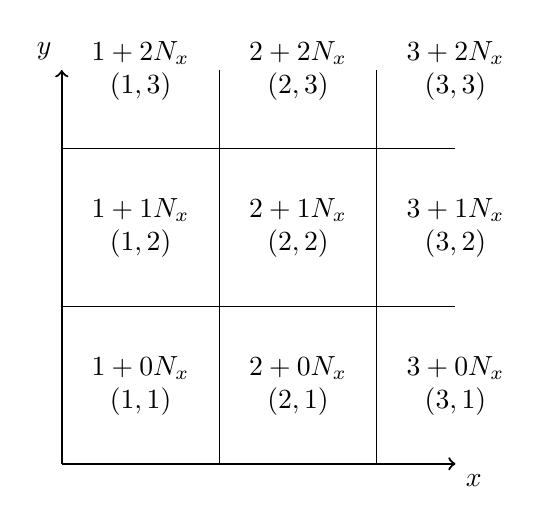
\begin{tikzpicture}
		\draw[step=2cm,black,thin] (0,0) grid (5,5);
		\draw[thick,->] (0,0) -- (5,0) node[anchor=north west] {$x$};
		\draw[thick,->] (0,0) -- (0,5) node[anchor=south east] {$y$};
		\foreach \x in {1,2,3}
			\pgfmathparse{\x*2-1}
			\edef\cx{\pgfmathresult}
			\foreach \y in {1,2,3}
				\pgfmathparse{\y*2-1}
				\edef\cy{\pgfmathresult}
				\pgfmathparse{int(\y-1)}
				\edef\ym{\pgfmathresult}
				\draw (\cx cm,\cy cm) node[anchor=center] {$\begin{matrix}\x+\ym N_x\\ (\x,\y)\end{matrix}$};
	\end{tikzpicture}
	\captionof{figure}[Caption]{Orientation of the coordinates and fields in the scene, with corresponding $\left(\begin{matrix}\text{1D} \\ \text{2D} \end{matrix}\right)$ cell indexing of the scene. The 1D notation is used to orient corresponding vectors and matrices, while the 2D notation is used for legibility and elementwise computations}
	\label{fig:indexing}
\end{figure}
This way, we discretize our fields to vectors $\gvec{\rho}^n,\vec{v_x}^n,\vec{v_y}^n, \vec{p}^n\in\mathbb{R}^{N_xN_y}$ for any time step $n\in\mathbb{N}$. The relation between a field $u$ and its discrete representation $\vec{u}^n$ is defined as
$$\vec{u}^n_{(i,j)} = u((i-0.5)\Delta x,(j-0.5)\Delta y,n\Delta t)$$
This way the entries of vector $\vec{u}$ are approximations at the centre of the corresponding cells.
\ \\
So for any discrete scalar field $\vec{u}$, the value in cell $(i,j)$ is denoted as $\vec{u}_{i+(j-1)N_x}$. To increase legibility, we introduce a corresponding notation for indexing the scalar field in $(i,j)$:
\begin{equation}
	\vec{u}_{(i,j)}:=\vec{u}_{i+(j-1)N_x}
\end{equation}
\subsection{Interpolation}
Before being able to discretize our density and velocity fields, we first need to interpolate them from individual agent positions. Let the scene contain $n$ agents, $a_1,\dots,a_n$, located at position $(x_{a_i},y_{a_i})$.
\ \\
The agents are modelled as Lagrangian particles. This means the agents have no volume, but their mass and velocity are concentrated into a single point.
In this implementation, we assume equal mass for all agents: $m_{a_i}=m = 1\ \forall i$. 
We convert an agents mass to a density by convolving with a two-dimensional Gaussian kernel $\phi(x,y)$ defined as 
\begin{equation}
	\label{eq:gaussian}
	\phi(x,y)=A \exp\left(-\left(\frac{x^2}{2\sigma_x^2}+\frac{y^2}{2\sigma_y^2}\right)\right)
\end{equation}
\emph{Currently, we are in the process of finding suited values for $A$, $\sigma_x$ and $\sigma_y$.}

\ \\
Let $\delta_{(x_0,y_0})$ be the Dirac distribution with value $\infty$ in $(x_0,y_0)$ and 0 everywhere else. Let $f*g$ be the convolution of $f$ and $g$. 
\ \\
Let agent $a_i$ be in location $(x_{a_i},y_{a_i})$ at time $t$. Then the density contribution $\rho_{a_i}(x,y)$ and velocity contribution $v_{a_i}(x,y)$ become
\begin{align}
	\rho_{a_i}(x,y) = m\delta*\phi\\
	v_{a_i}(x,y) = \begin{pmatrix}v_{a_i,x}\\v_{a_i,y}\end{pmatrix}\delta*\phi
\end{align}
Since $\phi$ is rotation symmetric, it can be expressed in polar coordinates:
\begin{align}
	r = \sqrt{\frac{x^2}{2\sigma_x^2}+\frac{y^2}{2\sigma_x^2}}\\
	\phi(r) = A\exp\left(-r^2\right).
\end{align}
We use a approximation of the Gaussian kernel called the Wendland-kernel \cite{violeau12}. This kernel is defined as follows:
\begin{equation}
	\label{eq:wendland}
	f_W(r) = \begin{cases}
				\left(1-\frac{r}{2}\right)^4(1+2r)& 0\leq r \leq 2\\
				0 & 2 < r 
			\end{cases}
\end{equation}
This approximation has some nice computational properties in comparison to other Gaussian approximation. We can reveal them by rewriting the expression to 
\begin{equation}
	f_W(r) = \max\left\{1-\frac{r}{2},0\right\}^4(1+2r)
\end{equation}
which is a single case function requiring only addition, multiplication, and a $\max$ function. This provides a welcome computational benefit, since a kernel convolution is a common operation in this implementation.

\ \\
To find the total density and total velocity in the cell centres for each cell, we sum over the densities and velocities of the agents in the (up to 8) neighbouring cells. This method is equivalent to the particle-in-cell method as described in \cite{zhu13}.\\
\begin{figure}[h]
	\centering
	\includegraphics[width=0.65\textwidth]{images/scene.png}
	\caption{Scene initiated with 1000 agents being directed to the exit south}
	\label{fig:cont_ex_scene}
\end{figure}
\begin{figure}[h]
	\centering
	\includegraphics[width=0.85\textwidth]{images/flow_fields.png}
	\caption{Continuous representation of the scene: density and velocity}
	\label{fig:cont_flow_field}
\end{figure}\\
In Figure \ref{fig:cont_ex_scene} we see an example scene with agents. In Figure \ref{fig:cont_flow_field} we see the corresponding density and velocity fields.
\subsection{Scheme}
\label{sec:scheme}
To discretize our partial differential equation we use a second order central difference scheme. So for scalar field $u$ we have the following gradient approximation:
\begin{align*}
\nabla u=\begin{pmatrix}\dfrac{\partial u}{\partial x}\\\dfrac{\partial u}{\partial y}\end{pmatrix}
=\begin{pmatrix}\dfrac{\vec{u}_{(i+1,j)}-\vec{u}_{(i-1,j)}}{2h_x}\\\dfrac{\vec{u}_{(i,j+1)}-\vec{u}_{(i,j-1)}}{2h_y}\end{pmatrix}+\bigo{h^2}.
\end{align*}
and for vector field $w$ we define the divergence approximation accordingly:
\begin{equation}
\nabla\cdot w=\dfrac{\partial w}{\partial x}+\dfrac{\partial w}{\partial y}=\dfrac{\vec{w}_{(i+1,j)}-\vec{w}_{(i-1,j)}}{2h_x}+\dfrac{\vec{w}_{(i,j+1)}-\vec{w}_{(i,j-1)}}{2h_y}+\bigo{h^2}.
\end{equation}
However, if we were to discretize $\nabla\cdot(\nabla u)$ this way, computing the value at cell $(i,j)$ would require cell values from non-adjacent neigbour cells. Therefore, when computing the divergence of the gradient, we use the more compact scheme:
\begin{equation*}
\nabla\cdot(\nabla u) = \dfrac{\vec{u}_{(i+1,j)}-2\vec{u}_{(i,j)}+\vec{u}_{(i-1,j)}}{h_x^2}+\dfrac{\vec{u}_{(i,j+1)}-2\vec{u}_{(i,j)}+\vec{u}_{(i,j-1)}}{h_y^2}+\bigo{h^2}
\end{equation*}
This way, we have ensured all terms of the PDE can be computed for every cell not on the boundary.

\ \\
To discretize in time, we use the explicit Euler method. This way we only need the values of the previous time step to compute the values of the next time step. This suits our system best, because after every iteration of the fluid flow solver, the scene has changed due to individual actions of agents. Therefore previous time steps have little practical information.

\ \\
Our resulting scheme is presented below:
\begin{equation}
	\begin{split}
		\dfrac{\gvec{\rho}^{n+1}_{(i,j)} - \gvec{\rho}^{n}_{(i,j)}}{\Delta t} =
		% div(\gvec{\rho}*v)\Delta t
		&-\dfrac{\gvec{\rho}^{n}_{(i+1,j)}\vec{v}^{n}_{x(i+1,j)}-\gvec{\rho}^{n}_{(i-1,j)}\vec{v}^{n}_{x(i-1,j)}}{2h_x} \\
		&-\dfrac{\gvec{\rho}^{n}_{(i,j+1)}\vec{v}^{n}_{y(i,j+1)}-\gvec{\rho}^{n}_{(i,j-1)}\vec{v}^{n}_{y(i,j-1)}}{2h_y}\\
		%div(\gvec{\rho}*\grad \vec{p})\Delta t
		&+\frac{1}{h^2_x}\left(\frac{1}{4}(\gvec{\rho}^{n}_{(i+1,j)}-\gvec{\rho}^{n}_{(i-1,j)})(\vec{p}^{n}_{(i+1,j)}-\vec{p}^{n}_{(i-1,j)})+ \gvec{\rho}^{n}_{(i,j)}(\vec{p}^{n}_{(i+1,j)}-2\vec{p}^{n}_{(i,j)}+\vec{p}^{n}_{(i-1,j)})\right)\\
		&+\frac{1}{h^2_y}\left(\frac{1}{4}(\gvec{\rho}^{n}_{(i,j+1)}-\gvec{\rho}^{n}_{(i,j-1)})(\vec{p}^{n}_{(i,j+1)}-\vec{p}^{n}_{(i,j-1)})+ \gvec{\rho}^{n}_{(i,j)}(\vec{p}^{n}_{(i,j+1)}-2\vec{p}^{n}_{(i,j)}+\vec{p}^{n}_{(i,j-1)})\right)
	\end{split}
	\label{eq:scheme}
\end{equation}
It is suitable to express our scheme in terms of matrices and vectors. Not only does this provide us with an efficient way to implement our scheme, it also sets us up for an efficient way of solving the PDE (as explained in Section \ref{sec:lcp})

\ \\
Before reformulating our scheme, we introduce \emph{Kronecker} products and vector gradients.
\subsubsection{Kronecker product}
Let $A \in \mathbb{R}^{m\times n}$ and $B \in \mathbb{R}^{p \times q}$. The Kronecker product $A\otimes B\in \mathbb{R}^{mp \times nq}$ is defined as
\begin{equation*}
	A\otimes B = \begin{pmatrix}
		a_{11}B &\cdots & a_{1n}B\\
		\vdots & \ddots & \vdots\\
		a_{m1}B & \cdots & a_{mn}B
	\end{pmatrix}.
\end{equation*}
The Kronecker product will prove valuable in notation and computation of our matrices.
% \subsubsection{Hadamard Product}
% Let $A \in \mathbb{R}^{m\times n}$ and $B \in \mathbb{R}^{m \times n}$. The Hadamard product $A\circ B\in \mathbb{R}^{m \times n}$ is the elementwise product of $A$ and $B$:
% \begin{equation*}
% 	A\circ B = \begin{pmatrix}
% 		a_{11}b_{11} &\cdots & a_{1n}b_{1n}\\
% 		\vdots & \ddots & \vdots\\
% 		a_{m1}b_{m1} & \cdots & a_{mn}b_{mn}
% 	\end{pmatrix}.
% \end{equation*}
% Each of the terms \eqref{eq:scheme1}, \eqref{eq:scheme1}, \eqref{eq:scheme3}, and \eqref{eq:scheme4} can be expressed separately by a combination of Kronecker products.
\subsubsection{Vector difference operator}
In Section \ref{sec:scheme} we defined the discretization of the gradient. We would like to compute a gradient for every cell in the scene, even for the boundary. We introduce a directional \emph{difference operator} that will aid us in computing the gradient approximation. First we surround our scene with a extra layer of cells. These virtual cells are meant to ensure the presence of 8 neighbour cells for all the cells in the scene. We fix the density and velocity in these virtual cells to 0. 
For a discrete field $\vec{u}\in \mathbb{R}^{N_xN_y}$ let the auxiliary extended field be denoted by $\vec{\tilde{u}} \in \mathbb{R}^{(N_x+2)(N_y+2)}$ defined such that:
\begin{equation}
	\vec{\tilde{u}}_{(i,j)} = \begin{cases}
		\vec{u}_{(i,j)}&\mbox{if } i \in \left\{ 1,\dots,N_x \right\},j \in \left\{ 1,\dots,N_y \right\} \\
		0&\mbox{else}
	\end{cases}.
	\label{def:gradient}
\end{equation}
We define our difference operators $\D_x, \D_y:\mathbb{R}^{N_xN_y}\to\mathbb{R}^{N_xN_y}$ as follows:
\begin{align*}
	\left( \D_x\vec{u} \right)_{(i,j)} &= \vec{\tilde{u}}_{(i+1,j)}-\vec{\tilde{u}}_{(i-1,j)}\\
	\left( \D_y\vec{u} \right)_{(i,j)}  &= \vec{\tilde{u}}_{(i,j+1)}-\vec{\tilde{u}}_{(i,j-1)}
	%&\forall i\in \left\{ 1,\dots,N_x \right\},\,\forall j \in \left\{ 1,\dots,N_y \right\}
\end{align*}
\subsubsection{Matrix composition}
We first define two tridiagonal matrices $P_{m},Q_{m}\in \mathbb{R}^{m\times m}$
\begin{align*}
	P_{m} &= \begin{pmatrix}
		0 & 1 &  & &  \\
		-1 & 0 & 1 &   &  \\
		  & -1 & \ddots & \ddots &  \\
		  &  & \ddots & \ddots &1 \\
		 & &  & -1 & 0
	\end{pmatrix}\\
	Q_{m} &= \begin{pmatrix}
		-2 & 1 &  & &  \\
		1 & -2 & 1 &   &  \\
		  & 1 & \ddots & \ddots &  \\
		  &  & \ddots & \ddots &1 \\
		 & &  & 1 & -2
	\end{pmatrix}
\end{align*}
Let $I_m$ be the identity matrix of rank $m$. Let $\diag:\mathbb{R}^n\to\mathbb{R}^{n\times n}$ be the operator that converts a vector $\vec{p}$ to a diagonal matrix:
\begin{equation}
	\diag(\vec{p}) = \begin{pmatrix}
		\vec{p}_1\\
		&\vec{p}_2\\
		&&\ddots\\
		&&&\vec{p}_n
	\end{pmatrix}.
	\label{def:diag}
\end{equation}
Finally we can define our scheme with two matrices for each divergence term in \eqref{eq:scheme}.
\begin{align*}
	A_x &= \frac{1}{4h_x^2}\diag(\D_x\gvec{\rho}^n)(P_{N_x}\otimes I_{N_y})\\
	A_y &= \frac{1}{4h_y^2}\diag(\D_y\gvec{\rho}^n)(I_{N_x}\otimes P_{N_y})\\
	B_x &= \frac{1}{h_x^2}\diag(\gvec{\rho})(Q_{N_x}\otimes I_{N_y})\\
	B_y &= \frac{1}{h_y^2}\diag(\gvec{\rho})(I_{N_x}\otimes Q_{N_y})
\end{align*}
Our final matrix $C$ becomes 
\begin{equation}
	C = A_x + A_y + B_x + B_y 
	\label{eq:total_matrix}
\end{equation}
We can define a vector $\vec{b}$ to express the \underline{velocity divergence} term:
\begin{equation}
	\vec{b} = -\left( \frac{1}{2h_x}\D_x(\vec{v}^n_{x(i,j)}\gvec{\rho}^n_{(i,j)}) + \frac{1}{2h_y}\D_y(\vec{v}^n_{y(i,j)}\gvec{\rho}^n_{(i,j)})\right)
	\label{def:vector}
\end{equation}
Combining \eqref{eq:total_matrix} and \eqref{def:vector} we obtain the following matrix-vector system
\begin{equation}
	\gvec{\rho}^{n+1}=\gvec{\rho}^{n}+(C\vec{p}^n + \vec{b})\Delta t.
	\label{eq:matr_vec_scheme}
\end{equation}

\section{Linear complementary problem}
\label{sec:lcp}
This system is linear in both $\vec{p}$ and $\gvec{\rho}$. Combining this with the complementarity between $\vec{p}$ and $\gvec{\rho}$ we can solve this system efficiently by reformulating it to fit a linear complementarity problem (LCP).
\subsection{Definition}
For matrix $M \in \mathbb{R}^{m\times n}$ and vector $\vec{q}\in \mathbb{R}^n$, a LCP has the following general form. Find $\vec{w},\vec{z}\in \mathbb{R}^m$ such that
\begin{align}
	\vec{w}=M\vec{z}+\vec{q}\\
	\vec{w}\geq\vec{0},\vec{z}\geq\vec{0}\\
w_iz_i=0\mbox{ for all }i
\label{def:lcp}
\end{align}
Positive semidefiniteness of $M$ is a sufficient condition to solve this problem, regardless of $q$.
We choose the following expressions:
\begin{align}
	\vec{w} &= \rho_{\max}-\gvec{\rho}^{n+1}\\
	\vec{q} &= \rho_{\max}-\gvec{\rho}^n+\left(\D_x(\gvec{\rho}^n\vec{v}^n)+\D_y(\gvec{\rho}^n\vec{v}^n)\right)\Delta t\\
	\vec{z} &= \vec{p}^n\\
	M &= C\Delta t\\
	\label{eq:lcp}
\end{align}
Using these expressions, we have reformulated our scheme to an LCP.
\emph{Here should follow some analysis as to why $C$ is not far from symmetric and positive definite. I used a minimum value on $\gvec{\rho}$ which should ensure positive eigenvalues on $C$.
I did some analysis on $C$ and found that the real part of all eigenvalues is positive and the matrix is 'almost' symmetric. I am not sure if it is doable to perform a theoretical analysis, but I could provide some plots and numerical eigenvalues\dots}
\subsection{Quadratic program}
There are several ways to solve linear complementary problems. If  matrix $M$ is positive definite, LCPs can be solved by a quadratic program (QP) solver, of which there exist many. Since we asserted $M$ to be positive definite, we rewrite our LCP to a quadratic program and solve it using the Python library \texttt{cxvopt} \cite{cvxopt}.
\ \\
Any LCP of the form \eqref{def:lcp} can be rewritten to a QP as follows: Minimize $f(\vec{z})$ where
\begin{equation}
	f(\vec{z}) = \vec{z}^T\left( M\vec{z}+\vec{q} \right)
\end{equation}
with the constraints:
\begin{align}
	M\vec{z} + \vec{q}\geq\vec{0}\\
	\vec{z}\geq\vec{0}
\end{align}
Note that these constraints assert $f(\vec{z}) \geq 0$. 

\ \\
$\vec{z}$ is a solution to our LCP if and only if $f(\vec{z})=0$. Should it be that due to numerical errors no such $\vec{z}$ can be found, we still yield a satisfying\footnote{verify this} approximation by having found a minimum for $f(\vec{z})$.
\subsection{Adjusting velocity with pressure}
We obtained our pressure term $\vec{p}^n$. We compute the gradient $\nabla\vec{p}^n$ and substract it from the velocity. After that, we normalize the velocity to $v_{\max}$.
The result is our final grid velocity $\tilde{v}^n$ satisfying
\begin{equation}
	\tilde{v}^n = \frac{\vec{v}^n-\nabla\vec{p}^n}{||\vec{v}^n-\nabla\vec{p}^n||}
	\label{eq:finvelocity}
\end{equation}
We use $\tilde{v}^n$ to steer the velocity of the agents. First we interpolate the final crowd velocity $\tilde{v}^n_{a_i}$ at the agents location $(x_{a_i},y_{a_i})$ by applying bilinear interpolation from the 4 surrounding cell values\footnote{check in implementation}. We determine the individual velocity $v^{n+1}_{a_i}$ by computing the weighted average as described in \eqref{eq:dens_velo}.
\newpage
\bibliographystyle{abbrv}
\bibliography{bib} 
\end{document}
